\chapter{Numbering Systems}
\graphicspath{ {./chapter01/FigWork} }

\section{Helpfull Stuff}

\begin{tabular}{|c|c|c|c|}\hline
Decimal & Binary & Hexadecimal \\ \hline
0	& 0000	& 0	 \\ \hline
1	& 0001	& 1	 \\ \hline
2	& 0010	& 2	 \\ \hline
3	& 0011	& 3	 \\ \hline
4	& 		& 4	 \\ \hline
5	& 0101	& 5	 \\ \hline
6	& 		& 6	 \\ \hline
7	& 		& 7	 \\ \hline
8	& 1000	& 8	 \\ \hline
9	& 		& 9	 \\ \hline
10	& 1010	& A	 \\ \hline
11	& 		& B	 \\ \hline
12	& 1100	& C	 \\ \hline
13	& 1101	& D	 \\ \hline
14	& 		& E	 \\ \hline
15	& 1111	& F	 \\ \hline
\end{tabular}
\vspace{0.5in}



\begin{tabular}{|c|c|c|c|c|c|c|c|c|c|c|}\hline
i    & 0 & 1 &  2 &  3 &  4 &  5 &  6 &  7  &  8  &  9  \\ \hline
$2^i$ & 1 & 2 &  4 &  8 & 16 & 32 & 64 & 128 & 256 &  512\\ \hline
\end{tabular}
\vspace{0.5in}

{\tiny
$\begin{array}{l}
1110101011_2= \\
1*2^9+1*2^8+1*2^7+0*2^6+1*2^5+0*2^4+1*2^3+0*2^2+1*2^1+1*2^0 = \\
2^8(0*2^3+0*2^2+1*2^1+1*2^0) + 2^4(1*2^3+0*2^2+1*2^1+0*2^0) + 2^0*(1*2^3+0*2^2+1*2^1+1*2^0) =\\
2^8(0011_2) + 2^4(1010_2) +  2^0(1011_2) =\\
2^{4*2}(0011_2) + 2^{4*1}(1010_2) +  2^{4*0}(1011_2) =\\
16^2(0011_2) + 16^1(1010_2) + 16^0*(1011_2) =\\
16^2(3) + 16^1(A) + 16^0*(B) =\\
3AB_{16}
\end{array}$
}


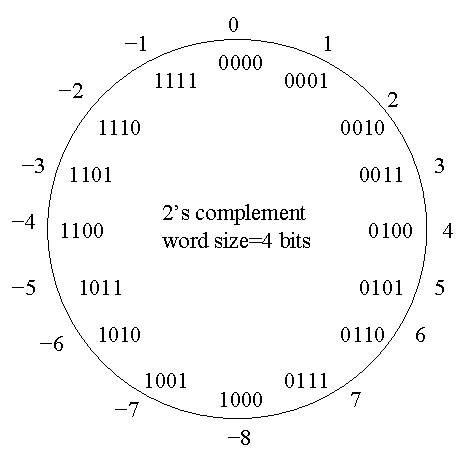
\includegraphics{../Fig/2wheel}


